% 1977 年四川卷第五题：梯形 ABCD，上底 AB=a、下底 DC=b、腰 AD=c、BC=d，
% a:b:c:d=1:3:1:2；角 α 在 C、角 β 在 D，虚线 AE、BF 为高，垂足 E、F（按源卷第 4 页布局）
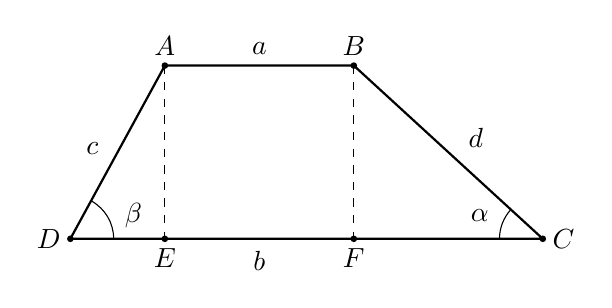
\begin{tikzpicture}[scale=1.0]
  \coordinate (D) at (0,0);
  \coordinate (C) at (6,0);
  \coordinate (A) at (1.2,2.2);
  \coordinate (B) at (3.6,2.2);
  \coordinate (E) at (1.2,0);
  \coordinate (F) at (3.6,0);
  \draw[thick] (D)--(C)--(B)--(A)--cycle;
  \draw[dashed] (A)--(E);
  \draw[dashed] (B)--(F);
  \fill (A) circle (1.2pt) node[above] {$A$};
  \fill (B) circle (1.2pt) node[above] {$B$};
  \fill (C) circle (1.2pt) node[right] {$C$};
  \fill (D) circle (1.2pt) node[left] {$D$};
  \fill (E) circle (1.2pt) node[below] {$E$};
  \fill (F) circle (1.2pt) node[below] {$F$};
  \node at (2.4,2.42) {$a$};
  \node at (2.4,-0.28) {$b$};
  \node at (0.28,1.15) {$c$};
  \node at (5.15,1.28) {$d$};
  % 角 β（D 处，DC 与 DA 之间）
  \draw (0.55,0) arc[start angle=0, end angle=61, radius=0.55];
  \node at (0.80,0.30) {$\beta$};
  % 角 α（C 处，CD 与 CB 之间）
  \draw ([shift={(6,0)}]137:0.55) arc[start angle=137, end angle=180, radius=0.55];
  \node at (5.20,0.30) {$\alpha$};
\end{tikzpicture}
